%%%%%%%%%%%%%%%%%%%%%%%%%%%%%%%%%%%%%%%%%
% KOMA-Script Presentation
% LaTeX Template
% Version 1.0 (3/3/13)
%
% This template has been downloaded from:
% http://www.LaTeXTemplates.com
%
% Original Authors:
% Marius Hofert (marius.hofert@math.ethz.ch)
% Markus Kohm (komascript@gmx.info)
% Described in the PracTeX Journal, 2010, No. 2
%
% License:
% CC BY-NC-SA 3.0 (http://creativecommons.org/licenses/by-nc-sa/3.0/)
%
%%%%%%%%%%%%%%%%%%%%%%%%%%%%%%%%%%%%%%%%%

%----------------------------------------------------------------------------------------
%	PACKAGES AND OTHER DOCUMENT CONFIGURATIONS
%----------------------------------------------------------------------------------------

\documentclass[
paper=A6,landscape,
%paper=128mm:96mm, % The same paper size as used in the beamer class
fontsize=11pt, % Font size
pagesize, % Write page size to dvi or pdf
parskip=half-, % Paragraphs separated by half a line
]{scrartcl} % KOMA script (article)

\linespread{1.12} % Increase line spacing for readability

%------------------------------------------------
% Colors
\usepackage{xcolor}	 % Required for custom colors
% Define a few colors for making text stand out within the presentation
\definecolor{mygreen}{RGB}{44,85,17}
\definecolor{myblue}{RGB}{34,31,217}
\definecolor{mybrown}{RGB}{194,164,113}
\definecolor{myred}{RGB}{255,66,56}
%\definecolor{MyDarkBlue}{rgb}{0,.2,.5}
\definecolor{MyDarkBlue}{RGB}{0,51,160}
\definecolor{nblue}  {RGB}{28,130,185}
% Use these colors within the presentation by enclosing text in the commands below
\newcommand*{\mygreen}[1]{\textcolor{mygreen}{#1}}
\newcommand*{\myblue}[1]{\textcolor{myblue}{#1}}
\newcommand*{\mybrown}[1]{\textcolor{mybrown}{#1}}
\newcommand*{\myred}[1]{\textcolor{myred}{#1}}
\newcommand*{\MyDarkBlue}[1]{\textcolor{MyDarkBlue}{#1}}
% My math symbols
\newcommand{\bfm}{{\mathbf m}}
\newcommand{\bfx}{{\mathbf m}}
\newcommand{\bfb}{{\mathbf d}}
\newcommand{\bfy}{{\mathbf y}}
\newcommand{\bfI}{{\mathbf I}}
\newcommand{\bfeps}{\mbox{{\boldmath$\epsilon$}}}
\newcommand{\bfdel}{\mbox{{\boldmath$\delta$}}}
\newcommand{\cov}{\textnormal{cov}}
%\newcommand{\bfd}{{\mathbf d}}
\newcommand{\bfd}{{\mathbf d}}
\newcommand{\bfsig}{\mbox{{\boldmath$\sigma$}}}
\newcommand{\bfrho}{\mbox{{\boldmath$\rho$}}}
\newcommand{\bfG}{{\mathbf G}}
\newcommand{\bfR}{{\mathbf R}}
\newcommand{\bfD}{{\mathbf D}}
\newcommand{\bfL}{{\mathbf L}}
\newcommand{\bfF}{{\mathbf F}}
\newcommand{\bfJ}{{\mathbf J}}
\newcommand{\bfC}{{\mathbf C}}
\newcommand{\bfA}{{\mathbf G}}
\newcommand{\bfW}{{\mathbf W}}
\newcommand{\eps}{{\epsilon}}
\newcommand{\bfr}{{\mathbf r}}
\newcommand{\bfnu}{\mbox{{\boldmath$\nu$}}}
\newcommand{\bfzero}{\mbox{{\boldmath$0$}}}
\newcommand{\argmin}{argmin}
\newenvironment{packed_enum}{
\begin{itemize}
  \setlength{\itemsep}{0pt}
  \setlength{\parskip}{0pt}
  \setlength{\parsep}{-2pt}
}{\end{itemize}}
%\DeclareMathOperator*{\argmin}{argmin}
\DeclareOldFontCommand{\bf}{\normalfont\bfseries}{\mathbf}
\DeclareOldFontCommand{\it}{\normalfont\itshape}{\mathit}
 \usepackage[cmex10]{amsmath}
 \usepackage{amssymb}
\usepackage{fixltx2e}
 \usepackage{stfloats}
  \usepackage{url}
  \usepackage[caption=false,font=footnotesize]{subfig}
  \usepackage{multirow}
  \usepackage{graphicx}
  \usepackage{multicol}
  \usepackage{array}
  \usepackage{amsmath}
  \usepackage{amsfonts}
%------------------------------------------------

%------------------------------------------------
% Margins
\usepackage[ % Page margins settings
includeheadfoot,
top=3.5mm,
bottom=3.5mm,
left=5.5mm,
right=5.5mm,
headsep=6.5mm,
footskip=8.5mm
]{geometry}
%------------------------------------------------

%------------------------------------------------
% Fonts
\usepackage[T1]{fontenc}	 % For correct hyphenation and T1 encoding
\usepackage{lmodern} % Default font: latin modern font
%\usepackage{fourier} % Alternative font: utopia
%\usepackage{charter} % Alternative font: low-resolution roman font
\renewcommand{\familydefault}{\sfdefault} % Sans serif - this may need to be commented to see the alternative fonts
%------------------------------------------------

%------------------------------------------------
% Various required packages
\usepackage{amsthm} % Required for theorem environments
\usepackage{bm} % Required for bold math symbols (used in the footer of the slides)
\usepackage{graphicx} % Required for including images in figures
\usepackage{tikz} % Required for colored boxes
\usepackage{booktabs} % Required for horizontal rules in tables
\usepackage{multicol} % Required for creating multiple columns in slides
\usepackage{lastpage} % For printing the total number of pages at the bottom of each slide
\usepackage[english]{babel} % Document language - required for customizing section titles
\usepackage{microtype} % Better typography
\usepackage{tocstyle} % Required for customizing the table of contents
%------------------------------------------------

%------------------------------------------------
% Slide layout configuration
\usepackage{scrpage2} % Required for customization of the header and footer
\pagestyle{scrheadings} % Activates the pagestyle from scrpage2 for custom headers and footers
\clearscrheadfoot % Remove the default header and footer
\setkomafont{pageheadfoot}{\normalfont\color{black}\sffamily} % Font settings for the header and footer

% Sets vertical centering of slide contents with increased space between paragraphs/lists
\makeatletter
\renewcommand*{\@textbottom}{\vskip \z@ \@plus 1fil}
\newcommand*{\@texttop}{\vskip \z@ \@plus .5fil}
\addtolength{\parskip}{\z@\@plus .25fil}
\makeatother

% Remove page numbers and the dots leading to them from the outline slide
\makeatletter
\newtocstyle[noonewithdot]{nodotnopagenumber}{\settocfeature{pagenumberbox}{\@gobble}}
\makeatother
\usetocstyle{nodotnopagenumber}

\AtBeginDocument{\renewcaptionname{english}{\contentsname}{\large Outline}} % Change the name of the table of contents
%------------------------------------------------

%------------------------------------------------
 %Header configuration - if you don't want a header remove this block
\ihead{
\hspace{-2mm}
\begin{tikzpicture}[remember picture,overlay]
\node [xshift=\paperwidth/2,yshift=-\headheight/2.1] (mybar) at (current page.north west)[rectangle,fill,inner sep=0pt,minimum width=\paperwidth,minimum height=.9\headheight,top color=MyDarkBlue!64,bottom color=MyDarkBlue]{}; % Colored bar
\node[below of=mybar,yshift=3.mm,rectangle,shade,inner sep=0pt,minimum width=128mm,minimum height =1.5mm,top color=black!50,bottom color=white]{}; % Shadow under the colored bar
shadow
\end{tikzpicture}}
%\color{white}\runninghead} % Header text defined by the \runninghead command below and colored white for contrast
%------------------------------------------------

%------------------------------------------------
% Footer configuration
%\newlength{\footheight}
\setlength{\footheight}{4mm} % Height of the footer
\addtokomafont{pagefoot}{\footnotesize} % Small font size for the footnote

\ifoot{% Left side
\hspace{-5.2mm}
%\begin{tikzpicture}[remember picture,overlay]
%\node [xshift=\paperwidth/2,yshift=\footheight] at (current page.south west)[rectangle,fill,inner sep=0pt,minimum width=\paperwidth,minimum height=3pt,top color=MyDarkBlue,bottom color=MyDarkBlue]{}; % Green bar
%\end{tikzpicture}
%\myauthor\ \raisebox{0.2mm}{$\bm{\vert}$}\ \myuni % Left side text
%\vspace{.01in}
\includegraphics[width=10cm,height=6mm]{footer.pdf} 
\includegraphics[width=2.cm]{logo.pdf}
}

%\ofoot[\pagemark/\pageref{LastPage}\hspace{-2mm}]{\pagemark/\pageref{LastPage}\hspace{-2mm}} % Right side
%------------------------------------------------

%------------------------------------------------
% Section spacing - deeper section titles are given less space due to lesser importance
\usepackage{titlesec} % Required for customizing section spacing
\titlespacing{\section}{0mm}{0mm}{0mm} % Lengths are: left, before, after
\titlespacing{\subsection}{0mm}{0mm}{-1mm} % Lengths are: left, before, after
\titlespacing{\subsubsection}{0mm}{0mm}{-2mm} % Lengths are: left, before, after
\setcounter{secnumdepth}{0} % How deep sections are numbered, set to no numbering by default - change to 1 for numbering sections, 2 for numbering sections and subsections, etc
%------------------------------------------------

%------------------------------------------------
% Theorem style
\newtheoremstyle{mythmstyle} % Defines a new theorem style used in this template
{0.5em} % Space above
{0.5em} % Space below
{} % Body font
{} % Indent amount
{\sffamily\bfseries} % Head font
{} % Punctuation after head
{\newline} % Space after head
{\thmname{#1}\ \thmnote{(#3)}} % Head spec
	
\theoremstyle{mythmstyle} % Change the default style of the theorem to the one defined above
\newtheorem{theorem}{Theorem}[section] % Label for theorems
\newtheorem{remark}[theorem]{Remark} % Label for remarks
\newtheorem{algorithm}[theorem]{Algorithm} % Label for algorithms
\makeatletter % Correct qed adjustment
%------------------------------------------------

%------------------------------------------------
% The code for the box which can be used to highlight an element of a slide (such as a theorem)
\newcommand*{\mybox}[2]{ % The box takes two arguments: width and content
\par\noindent
\begin{tikzpicture}[mynodestyle/.style={rectangle,draw=MyDarkBlue,thick,inner sep=2mm,text justified,top color=white,bottom color=white,above}]\node[mynodestyle,at={(0.5*#1+2mm+0.4pt,0)}]{ % Box formatting
\begin{minipage}[t]{#1}
#2
\end{minipage}
};
\end{tikzpicture}
\par\vspace{-1.3em}}
%------------------------------------------------

%----------------------------------------------------------------------------------------
%	PRESENTATION INFORMATION
%----------------------------------------------------------------------------------------

\newcommand*{\mytitle}{Regularization as Constrained Inversion } % 
%\newcommand*{\runninghead}{\footnotesize SIAM Imaging 2016 - Regularization Operators} % Running head displayed on almost all slides
\newcommand*{\myauthor}{Jodi Mead \hspace*{1.in} James Ford} % Presenters name(s)
\newcommand*{\myauth}{Diego Domenzain \hspace*{.85in} John Bradford} % Presenters name(s)
\newcommand*{\mydate}{\today} % Presentation date
\newcommand*{\myuni}{Boise State University} % University or department
\newcommand*{\mydept}{Department of Mathematics \hspace*{.5in} Clearwater Analytics} % University or department
\newcommand*{\myd}{Department of Geosciences \hspace*{.15in} Department of Geophysics} % University or department
\newcommand*{\mydj}{Colorado School of Mines}

%----------------------------------------------------------------------------------------

\begin{document}

%----------------------------------------------------------------------------------------
%	TITLE SLIDE
%----------------------------------------------------------------------------------------

% Title slide - you may have to tweak a few of the numbers if you wish to make changes to the layout
\thispagestyle{empty} % No slide header and footer
\begin{tikzpicture}[remember picture,overlay] % Background box
\node [xshift=\paperwidth/2,yshift=\paperheight/1.4] at (current page.south west)[rectangle,fill,inner sep=0pt,minimum width=\paperwidth,minimum height=\paperheight/3,top color=MyDarkBlue,bottom color=MyDarkBlue]{}; % Change the height of the box, its colors and position on the page here
\end{tikzpicture}
% Text within the box
\begin{flushright}
\vspace{-1.5cm}
\color{white}\sffamily
{\bfseries\large\mytitle\par} % Title
%\vspace{0.5cm}
\small
\myauthor\par% Author name

\vspace*{-.15in}

\mydept\par
\vspace*{-.1in}
\myauth\par% Author name

\vspace*{-.15in}

\myd\par

\vspace*{-.15in}
\mydj
%\vspace*{-.15in}
%\myuni\par % Date
\vfill
\end{flushright}

 
\hspace*{2.7in} Thanks to:   NSF DMS-1418714

\vspace{-.2in} 

\includegraphics[width=4.5cm]{logo_blue.pdf}  




\clearpage

%----------------------------------------------------------------------------------------
%	TABLE OF CONTENTS
%----------------------------------------------------------------------------------------

%\thispagestyle{empty} % No slide header and footer

%\vspace*{-0.7in}

%\small\tableofcontents % Change the font size and print the table of contents - it may be useful to shrink the font size further if the presentation is full of sections
% To exclude sections/subsections from the table of contents, put an asterisk after \(sub)section like so: \section*{Section Name}

%\vspace*{-0.3in}

%\clearpage

%----------------------------------------------------------------------------------------
%	PRESENTATION SLIDES
%----------------------------------------------------------------------------------------
%%--------------------------------------------------

{\large \bf Outline}
\begin{itemize}
\item Near subsurface imaging  of the Earth
\item Electrical Resistivity Tomography using Tikhonov regularization
\begin{itemize}
\item Regularization informed by data constraints
\end{itemize}
\item Assessing effectiveness of combining different data types
\item Results from combining Electrical Resistivity and Ground Penetrating Radar data
\end{itemize}
\clearpage
%%--------------------------------------------------

{\large \bf Near subsurface imaging}

\vspace*{.1in}

\centerline{ \it Boise Hydrogeophysical Research Site (BHRS)}
\vspace*{-.1in}
\begin{multicols}{2}
\vspace*{.0in}
\centerline{\resizebox{5.cm}{!}{\includegraphics{researchtop}}}
\columnbreak
\begin{packed_enum}
\item  Field laboratory on a gravel bar adjacent to the Boise River, 15 km southeast of downtown Boise.
\item Consists of coarse cobble and sand.  Braided stream fluvial deposits overlie a clay layer at about 20 m depth.
\end{packed_enum}
\end{multicols}
\vspace*{-.2in}

Difference in retention properties in a lenticular sand feature yields significantly different geophysical properties.


\clearpage
%%--------------------------------------------------

{\large \bf Electrical Resistivity Tomography (ERT)}

\vspace*{.1in}


\begin{multicols}{2}
\vspace*{.0in}
\centerline{\resizebox{5.cm}{!}{\includegraphics{ERT}}}
\columnbreak
\begin{packed_enum}
\item  2D grid of observations provides a 2.5-D inverted model that emphasizes the sand lenticular feature.
\item BHRS survey consisted of 12 electrodes spaced 1 meter apart acquired with a dipole-dipole configuration.
\end{packed_enum}
\end{multicols}
\vspace*{-.2in}

BHRS survey acquired at surface when subsurface achieved saturation.



\clearpage

%%--------------------------------------------------
\vspace*{-.5in}

{\large \bf Electrical Resistivity Model}
\vspace*{-.1in}
\begin{multicols}{2}
\centerline{\resizebox{4.cm}{!}{\includegraphics{ER_diego}}}
\columnbreak
%\vspace*{-.2in}
\begin{align*}
%\vspace*{-.2in}
%\hspace*{-.2in}
-\nabla\cdot\sigma\nabla \varphi = {\bf i}(\delta(x-s_+)-\delta(x-s_-)) \footnote{\footnotesize Pidlisecky and Knight, 2008}
%\vspace*{-.2in}
\end{align*}
$\varphi$ - electric potential\\
 ${\bf i}$ - current intensity \\ $s_{\pm}$ - source-sink position.
%\vspace*{-.2in}
\end{multicols}
%\vspace*{-.2in}
\begin{tabbing}
{\bf Model parameters:} \ \  \= conductivity $\sigma$ or resistivity $\rho=1/\sigma$\\

{\bf Observed data:}  \ \ \> apparent resitivity $ \frac{2\pi\triangle \varphi}{i} \kappa$
\end{tabbing}
\underline{\hspace*{2.in}} \\
$^1$Pidlisecky and Knight, 2008
%$ \kappa$ - geometrical information about electrodes
\clearpage


%%--------------------------------------------------
\vspace*{-.5in}

{\large \bf Tikhonov Regularization}
\[   \min_{\bfsig} \ \left\{ \| \bfd- F( \bfsig) \|_2^2 + \alpha^2 \|L_p \bfsig \|_2^2\right\} \] 
\centerline{$\alpha$-  regularization parameter, \ \ \   
$ L_p $ - 0th, 1st or 2nd derivative operator}

\vspace*{.2in}

	\centerline{True resistivity} \centerline{\resizebox{7.cm}{!}{ \includegraphics{topo_linear_model_L1_occam2_200040040001000_st_true_model.eps}}}
	
	\centerline{Inverted resistivity with $L_1$ \ \ \ \ \ \ \ \ \ \ \ \ \ \ \ \ \ \ \  Inverted resistivity with $L_2$}
	\centerline{\resizebox{7.cm}{!}{\includegraphics{topo_linear_model_L1_occam2_200040040001000_st_inv_model.eps}} 
	{\resizebox{7.cm}{!}{\includegraphics{topo_linear_model_L2_occam2_200040040001000_st_inv_model.eps}}}}

\clearpage


%%--------------------------------------------------
{\large \bf  Relaxing the Constraint}\\
\[   \min_{\bfsig} \ \left\{ \| \bfd- F( \bfsig) \|_2^2 + \alpha^2 \|RL_p \bfsig \|_2^2\right\} \] 
\hspace*{1.5in} {$R= \mbox{diag} (r_1,\ldots , r_n), \ r_i=0$ or $1$} \footnote{\footnotesize Hetrick and M., 2018}



	\centerline{$R$ } \centerline{\resizebox{4.cm}{!}{ \includegraphics{diagR}}}
	
	\centerline{Inverted resistivity with $RL_1$ \ \ \ \ \ \ \ \ \ \ \ \ \ \ \ \ \ \ \  Inverted resistivity with $RL_2$}
	\centerline{\resizebox{7.cm}{!}{\includegraphics{topo_linear_model_L1_occam2_200040040001000_R_inv_model.eps}} 
	{\resizebox{7.cm}{!}{\includegraphics{topo_linear_model_L2_occam2_200040040001000_R_inv_model.eps}}}}

\clearpage


%%--------------------------------------------------

\vspace*{-.5in}

{\large \bf Constraint - Ground Penetrating Radar (GPR)}

\begin{multicols}{2}
\vspace*{.0in}
\centerline{\resizebox{5.cm}{!}{\includegraphics{gpr}}}
\columnbreak
\begin{packed_enum}
\item  GPR survey at BHRS acquired across center of gridded ER survey.
 \item GPR sampled line collinear with ER survey.
\item GPR derived boundary gives constraint for inverting the ER dataset.
\end{packed_enum}
\end{multicols}
\clearpage
%%--------------------------------------------------


{\large \bf Boise Hydrogeophysical Research Site Results}


\begin{itemize}
\item ER data inverted for resistivity
\item Regularization in the form of
subsurface boundary constraint inferred from GPR data
\end{itemize}

\centerline{\resizebox{10.cm}{!}{\includegraphics{bhrsresults}}}
\clearpage
%%--------------------------------------------------


{\large \bf Summary -  Constraints as Tikhonov regularization}
\begin{itemize}
\item Additional data can be used to inform the regularization operator
\begin{itemize}
\item Initial parameter estimates, or their first or second derivatives,  can always produce a well-posed problem.
\item Adding derivative information only requires knowledge of where parameter values change, rather than parameter values.
\item May rely on secondary data processing or practitioner interpretation of data.
\end{itemize}
\end{itemize}
\clearpage
%--------------------------------------------------
{\large \bf Assessing Effectiveness of Constraints - Singular Value Expansion}\\
\[ \min_x \| d-Ax  \|_2^2 \]
with solution 
\[ x = A^{\dagger} b = \sum_{k=1}^{\infty} \frac{\langle \psi_k , b \rangle }{\sigma_k} \phi_k \]
%Condition number:    $\sigma_k \rightarrow 0$, as $k \rightarrow \infty$  
\centerline{ $\psi_k$, $\phi_k$ orthonormal singular functions}
\centerline{
$\sigma_k \rightarrow 0 \ \mbox{as} \ k \rightarrow \infty$}
\begin{itemize}
\item{Conditioning measured by decay rate of singular values}
\begin{itemize}
\item e.g.\ decay rate $q \Rightarrow \sigma_{k}$ decays like $k^{-q}$
\end{itemize}
\end{itemize}

\clearpage
%--------------------------------------------------
{\large \bf Singular Values of Tikhonov Operator}
\[%\min_x \left\Vert T_{\alpha}x-(b,0)\right\Vert _2^{2}=
\min_x\left\Vert d-Ax\right\Vert _2^{2}+\alpha^2 \left\Vert x\right\Vert _2^{2}
\]

%i.e\ $
%T_{\alpha}x=(Ax,\alpha^2 x) $\footnote{\footnotesize Gockenbach, 2015}.
with solution 
\[
x= A_{\alpha}^{\dagger}b=\sum_{k=1}^{\infty}\frac{\sigma_{k}}{\sigma_{k}^{2}+\alpha^2}\langle \psi_k , b \rangle \phi_{k}
\]
so that  
\[
\frac{\sigma_{k}}{\sigma_{k}^{2}+\alpha^2}\rightarrow0,\text{ as }k\rightarrow\infty
\]
and $\alpha$ restricts the solution space\footnote{\footnotesize Gockenbach, 2015}.

\clearpage
%--------------------------------------------------
{\large \bf Additional Data as Constraints}\\
\[
\left\Vert d_1-Ax\right\Vert _2^{2}+\left\Vert d_2-Bx\right\Vert _2^{2}
\]
Singular values satisfy
\[   A^{*}A\phi+B^{*}B\phi =\sigma^{2}\phi  \ \  \ \ \mbox{or} \ \ \ \  C^{*}C\phi= \sigma^{2}\phi\]
and can be approximated with a Galerkin method  e.g.\ $A^{(n)}$,  $a_{ij}^{(n)}  = \langle q_i, Ap_j \rangle \nonumber $, where  $\{q_i(s)\}_{i=1}^{n}$ and $\{p_j(t)\}_{j=1}^{n}$  are orthonormal bases so that $$A^{(n)}=U^{(n)}\Sigma^{(n)}\left(V^{(n)}\right)^T, \ \ \ \Sigma^{(n)}=\text{diag}\left(\sigma_1^{(n)}, \sigma_2^{(n)}, \dots \sigma_n^{(n)}\right)$$
Define
$$C^{(n)}=\begin{bmatrix} A^{(n)}\\ B^{(n)} \end{bmatrix}$$
\clearpage
%--------------------------------------------------
{\large \bf Special case: Self-Adjoint Operators }

Use singular functions in Galerkin method
$$a_{ij}^{(n)}= \langle \phi_j, A \phi_i \rangle   =  \langle \phi_j, \sigma_i \phi_i \rangle  =   \left\{ \begin{array}{ll} \sigma_i & i=j \\ 0 & i \neq j \end{array} \right. $$
then $$A^{(n)}= \Sigma_A^{(n)} \ \  \mbox{and} \ \  B^{(n)}= \Sigma_B^{(n)}$$ so that
\[ \left( C^{(n)} \right)^T \left( C^{(n)} \right) = \left( \Sigma_A^{(n)}\right)^2 + \left( \Sigma_B^{(n)}\right)^2 \] and
\[\sigma_i \left( C^{(n)} \right) = \sqrt{\sigma_i \left( A^{(n)} \right)^2 + \sigma_i \left( B^{(n)} \right)^2}\]
\clearpage
%--------------------------------------------------
%{\large \bf Joint Singular Value Example}
%\begin{align*}
%L_{A}u & =  -u'', \quad	u(0)=u(\pi)=0,\\
%L_{B}u & =  u''+b^{2}u,	\quad u(0)=u(\pi)=0, \quad\text{and } b\notin \mathbb{Z}
%\end{align*}
%Green's functions:
%\[ K_{A}=\begin{cases}
%\frac{1}{b}\left(\pi-x\right)y, & 0\leq y\leq x\leq \pi,\\
%\frac{1}{b}\left(\pi-y\right)x, & 0\leq x\leq y\leq \pi.
%\end{cases}
%\]
%
%\[
%K_{B}= \begin{cases} -\frac{\sin(by)\sin[b(\pi-x)]}{b\sin(b\pi)}, & 0\leq y \leq x \leq \pi, \\
%-\frac{\sin(bx)\sin[b(\pi-y)]}{b\sin(b\pi)}, & 0\leq x \leq y \leq \pi.
%\end{cases}\]
%\clearpage
%%--------------------------------------------------
%{\large \bf Individual Singular Values - $b=\pi$ }
%
%\vspace*{.2in}
%
%\centerline{
%\includegraphics[height=1.45in]{svcont1}
%\includegraphics[height=1.45in]{svcont2}}
%
%\centerline{\hspace*{.2in}$\sigma_{k}(A^{(200)})=\frac{1}{k^{2}}$ \hspace*{.8in} $\sigma_{k}(B^{(200)})= \frac{1}{k^{2}+\pi^{2}}$}
%
%\clearpage
%%--------------------------------------------------
%{\large \bf Joint Singular Values -  $b=\pi$ }
%
%\vspace*{.2in}
%
%\centerline{
%\includegraphics[height=1.85in]{svcont3}
%\includegraphics[height=1.85in]{svcont4}}
%
%%\vspace*{.2in}
%
%\centerline{$\sigma_{k}(C^{(200)})=\sqrt{\left(\frac{1}{k^{2}}\right)^2 + \left(\frac{1}{k^{2}+\pi^{2}}\right)^2}$}
%\clearpage
%%--------------------------------------------------
%{\large \bf Joint Singular Values }
%
%\vspace*{.2in}
%
%\centerline{$b=10.1$  \hspace*{1.4in} $b=0.1$}
%\centerline{
%\includegraphics[height=1.45in]{svcont5}
%\includegraphics[height=1.45in]{svcont6}}
%
%\vspace*{.2in}
%
%\centerline{\small $\sigma_{k}(C^{(200)})=\sqrt{\left(\frac{1}{k^{2}}\right)^2 + \left(\frac{1}{k^{2}+10.1^{2}}\right)^2}$ \hspace*{.1in} $\sigma_{k}(C^{(200)})=\sqrt{\left(\frac{1}{k^{2}}\right)^2 + \left(\frac{1}{k^{2}+0.1^{2}}\right)^2}$}
%
%\clearpage
%--------------------------------------------------
{\large \bf Summary - Additional Data as Constraints }
\begin{itemize}
\item Data as constraints will reduce the amount of regularization necessary to resolve ill-posedness.
\begin{itemize}
\item However, adding data may not improve decay rate in individual inversions.
\end{itemize}
\item Singular values from theoretical models indicate properties and or situations where different data types effectively regularize each
other.
\end{itemize}
\clearpage
%%--------------------------------------------------

\vspace*{-.5in}

{\large \bf Complementary data in Subsurface Imaging}
\begin{multicols}{2}
\centerline{\underline{Ground Penetrating Radar}}
\begin{itemize} \item \small {High frequency}
\item \small Conductivity through \\ attenuation and reflection
\end{itemize}
\vspace*{.2in}
\centerline{\resizebox{6.cm}{!}{\includegraphics{gpr_compare}}}
\columnbreak	
\centerline{\underline{Electrical Resistivity}}
\begin{itemize} \item \small Low frequency
\item \small Directly sensitive to conductivity
\end{itemize}
\vspace*{.2in}
\centerline{\resizebox{4.cm}{!}{\includegraphics{er_compare}}}
\end{multicols}
\clearpage
%%--------------------------------------------------

\vspace*{-.5in}

{\large \bf GPR Model}
\vspace*{-.2in}
\begin{multicols}{2}
\vspace*{.0in}
\centerline{\resizebox{4.cm}{!}{\includegraphics{GPR_diego}}}
\columnbreak	
\vspace*{-.4in}
\begin{align*}
\varepsilon \ddot{u} + \sigma \dot{u} = \frac{1}{\mu} \nabla^2 u + s_w \footnote{\footnotesize Yee, 1966; Berenger, 1994, Ernst et al., 2007}
\end{align*}
$u$-electric field, ${\varepsilon}$-permittvity  \\$\mu$-constant permeability\\ $s_w$-source wavelet
%\vspace*{-.2in}
%\begin{align*}
% u &=  L_w s_w\\
%d_w &= M_w u
%\end{align*}
%\vspace*{-.2in}
\end{multicols}

\vspace*{-.2in}
\begin{tabbing}
{\bf Model parameters:} \ \  \= conductivity $\sigma$ and permitivity $\bfeps$\\
{\bf Observed data:}  \ \ \> electric current $Mu$
\end{tabbing}

%\vspace*{-.2in}
%Forward  model:   {\it finite difference time domain} on a Yee grid with PML% to solve for $d_w$
%.\footnote{\footnotesize Yee, 1966; Berenger, 1994}\\
%Inverse model: {\it full waveform inversion} to solve for $\varepsilon$ and $\sigma$.\footnote{\footnotesize Ernst et al., 2007}
\clearpage



%%--------------------------------------------------
\vspace*{-.5in}

{\large \bf Inverting ER and GPR jointly - full physics}

\centerline{\resizebox{9.cm}{!}{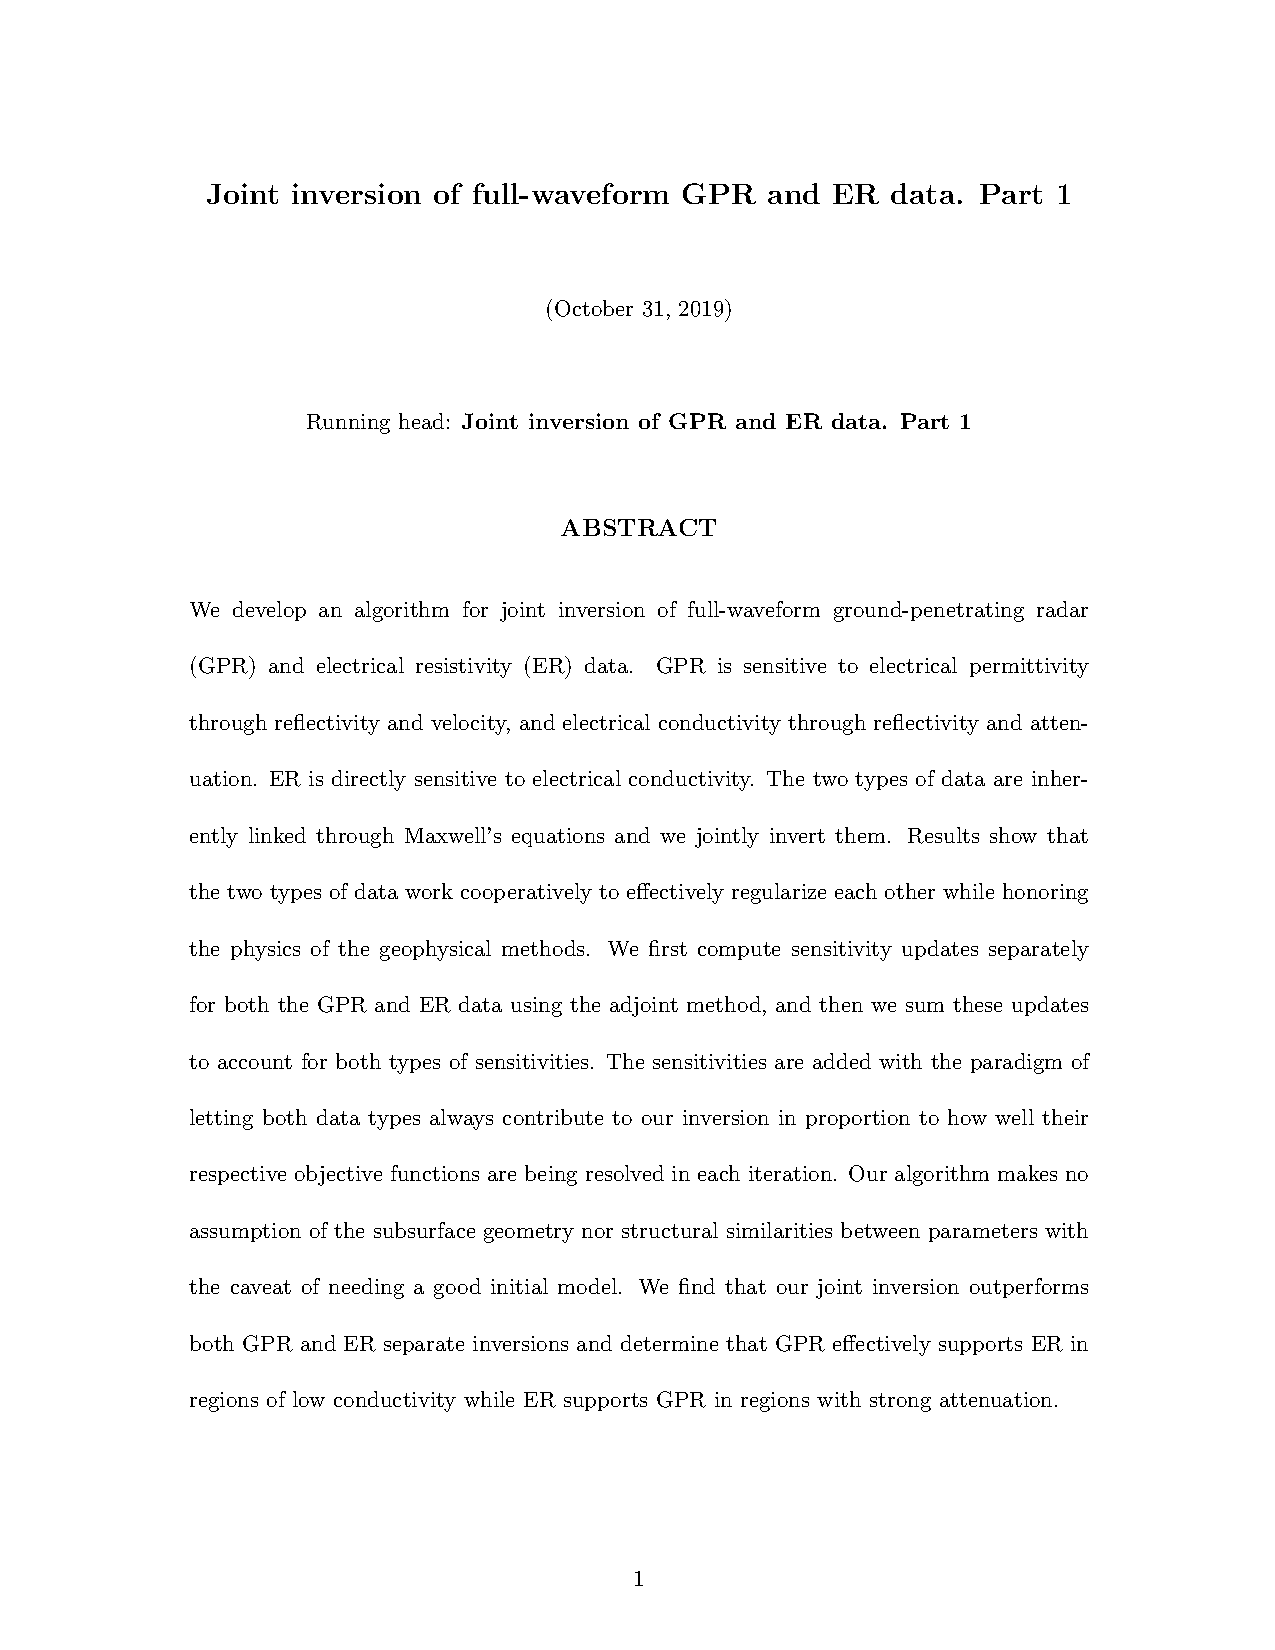
\includegraphics{joint}}}
\clearpage
%--------------------------------------------------
{\large \bf Combining updates}

\vspace*{.2in}
\centerline{\resizebox{8.cm}{!}{\includegraphics{updates}}}
\clearpage
%--------------------------------------------------
{\large \bf Data weights}

\vspace*{.2in}
\centerline{\resizebox{8.cm}{!}{\includegraphics{weights}}}
\clearpage

%--------------------------------------------------
{\large \bf Inverted images - full physics }

\centerline{\resizebox{7.cm}{!}{\includegraphics{joint_results}}}


\clearpage
%--------------------------------------------------
{\large \bf Inverted cross section - full physics}

\vspace*{.2in}
\centerline{\resizebox{9.cm}{!}{\includegraphics{cross_results}}}
\clearpage
%%--------------------------------------------------


{\large \bf Summary - \\ Jointly inverting two different data types with full physics}
\begin{itemize}
\item We have developed a joint inversion algorithm to solve for
both permittivity $\epsilon$ and conductivity $\sigma$   using complementary GPR and ER data.
\item Features were recovered that neither GPR or ER can individually resolve.
%\item Data weights must reflect the physics that can be captured by each particular data set during iterations of the inversion.
\item Future work will quantify the effectiveness of combining these data types 
\begin{itemize}
\item Calculate decay rate of singular values of individual and joint operators
\end{itemize}
\end{itemize}
\clearpage

%%--------------------------------------------------



{\large \bf Thank you!}
\vspace*{1.in}
\begin{flushright} Jodi Mead\\Mathematics Department\\ Boise State University\\ jmead@boisestate.edu \end{flushright}

\clearpage
%%--------------------------------------------------


\end{document}